\subsection{Manipulation 1 : Réglage du collimateur (image à l'infini)}

\subsubsection{Calcul de l'incertitude par méthode différentielle}

Pour évaluer la précision sur la mesure de $f'_1$,
nous utilisons la méthode des différentielles.
En partant de la relation de conjugaison de Descartes :
\begin{equation}
    \frac{1}{f'_1} = \frac{1}{p'} - \frac{1}{p}
\end{equation}

\paragraph{Expression de la différentielle}
En différenciant chaque terme de l'égalité, on obtient :
\begin{equation}
    d\left(\frac{1}{f'_1}\right) = d\left(\frac{1}{p'}\right) - d\left(\frac{1}{p}\right)
\end{equation}
\begin{equation}
    -\frac{df'_1}{{f'_1}^2} = -\frac{dp'}{{p'}^2} + \frac{dp}{p^2}
\end{equation}

Pour obtenir l'incertitude absolue $\Delta f'_1$,
on passe aux valeurs absolues afin de majorer l'erreur
(somme des erreurs maximales possibles) :
\begin{equation}
    \frac{\Delta f'_1}{{f'_1}^2} = \frac{\Delta p'}{{p'}^2} + \frac{\Delta p}{p^2}
\end{equation}

\paragraph{Formule finale}
On en déduit l'expression de l'incertitude absolue sur la focale :
\begin{equation}
    \Delta f'_1 = {f'_1}^2 \left( \frac{\Delta p'}{{p'}^2} + \frac{\Delta p}{p^2} \right)
\end{equation}

\subsubsection{Calcul de la valeur de la focale}

D'après les mesures relevées sur le banc optique :
\begin{itemize}
    \item Position de l'objet : $x_{obj} = 15,0$ cm
    \item Position de la lentille : $x_{L1} = 25,0$ cm
    \item Distance objet-lentille : $p = -10,0$ cm
    \item Distance lentille-écran : $p' = +175,0$ cm
\end{itemize}

La valeur expérimentale est calculée par :
\begin{equation}
    f'_1 = \left( \frac{1}{175} + \frac{1}{10} \right)^{-1} \approx 9,46 \text{ cm}
\end{equation}

L'application numérique de l'incertitude,
avec $\Delta p \approx \Delta p' \approx 0,2$ cm, donne :
\begin{equation}
    \Delta f'_1 = 10^2 \left( \frac{0,2}{175^2} + \frac{0,2}{10^2} \right) \approx 0,2 \text{ cm}
\end{equation}

\subsubsection{Résultats}

Voici le tableau des mesures et résultats pour la collimation :

\begin{center}
\begin{tabular}{|c|c|}
    \hline
    $f'_1$ (cm) & $\Delta f'_1$ (cm) \\
    \hline
    $9,5$ & $0,2$ \\
    \hline
\end{tabular}
\end{center}

\subsection{Expérience : Autocollimation}

\subsubsection{Mesures brutes}
Les positions relevées sur le banc optique sont les suivantes : 
\begin{itemize}
    \item Position de l'objet : $x_{obj} = 15,0 \pm 0,1$ cm 
    \item Position de la lentille : $x_{L} = 25,2 \pm 0,1$ cm 
\end{itemize}
La distance focale expérimentale est déduite par la relation $f'_{1} = |x_{L} - x_{obj}|$, 
ce qui donne $f'_{1} = 10,2$ cm. 

\subsubsection{Calcul d'incertitude}
La détermination de l'incertitude sur la distance focale $f'_{1}$ repose sur la méthode des différentielles appliquée à la relation de conjugaison de l'autocollimation. 
On considère la relation fonctionnelle : 
\[ f'_{1} = x_{L} - x_{obj} \] 
La différentielle totale de cette expression s'écrit : 
\[ df'_{1} = \frac{\partial f'_{1}}{\partial x_{L}}dx_{L} + \frac{\partial f'_{1}}{\partial x_{obj}}dx_{obj} = 1 \cdot dx_{L} - 1 \cdot dx_{obj} \] 
En passant aux incertitudes absolues, on somme les contributions des erreurs liées à chaque pointé : 
\[ \Delta f'_{1} = |1| \Delta x_{L} + |-1| \Delta x_{obj} = \Delta x_{L} + \Delta x_{obj} \] 
Les sources d'erreurs identifiées pour chaque position sont : 
\begin{itemize}
    \item L'erreur de lecture sur le banc optique : $\Delta x_{lect} = 0,1$ cm.
    \item La latitude de mise au point sur la position de la lentille : $\Delta x_{map} = 0,2$ cm. 
\end{itemize}
Ainsi, nous avons : 
\begin{itemize}
    \item $\Delta x_{L} = \Delta x_{lect} + \Delta x_{map} = 0,1 + 0,2 = 0,3$ cm. 
    \item $\Delta x_{obj} = \Delta x_{lect} = 0,1$ cm. 
\end{itemize}
L'incertitude absolue totale est donc : 
\[ \Delta f'_{1} = 0,3 + 0,1 = 0,4 \text{ cm.} \]

\subsubsection{Tableau des résultats}
Voici les résultats synthétisés ci-dessous : 

\begin{table}[h]
    \centering
    \begin{tabular}{|c|c|}
        \hline
        $f'_{1}$ (cm) & $\Delta f'_{1}$ (cm) \\
        \hline
        10,2 & 0,4 \\
        \hline
    \end{tabular}
    \caption{Distance focale de la lentille $L_1$ et son incertitude par la méthode d'autocollimation.}
\end{table}

\subsection{Méthode de Silbermann}

\subsubsection{Mesures brutes}
Lors de cette manipulation, 
nous avons déplacé conjointement la lentille et l'écran 
afin d'obtenir une image de même taille que l'objet, mais renversée. 
Les positions relevées sur le banc optique millimétré sont les suivantes :
$p = -20{,}0 \text{ cm}$
$p' = 20{,}0 \text{ cm}$

Ces mesures sont en parfait accord avec la théorie. 
En effet, d'après la relation de position de l'image démontrée dans la partie théorique, 
la condition $D=4f'$ implique que $|p| = |p'| = 2f'$. 
Ici, nous observons bien que l'objet et l'image 
sont situés à la même distance du centre optique de la lentille ($20{,}0 \text{ cm}$), 
ce qui correspond à un grandissement transversal $\gamma = \frac{p'}{p} = -1$.

\subsubsection{Calcul d'incertitude}
L'incertitude sur la distance focale $\Delta f'_1$ est calculée 
à partir de l'incertitude sur la distance objet-écran $D = p' - p$.
Pour un banc millimétré, l'incertitude de lecture est de $0{,}1 \text{ cm}$ par position.
$\Delta D = \Delta p' + \Delta p = 0{,}1 + 0{,}1 = 0{,}2 \text{ cm}$.

En appliquant la méthode des différentielles à la relation de Silbermann $f' = \frac{D}{4}$, 
nous obtenons l'expression suivante :
$\Delta f'_1 = \frac{\Delta D}{4} = \frac{0{,}2}{4} = 0{,}05 \text{ cm}$.

\subsubsection{Calcul de la distance focale image}
La distance focale est déterminée en utilisant la relation spécifique 
à la méthode de Silbermann établie dans la partie théorique :
$f'_1 = \frac{D}{4}$
$f'_1 = \frac{p' - p}{4} = \frac{20{,}0 - (-20{,}0)}{4} = \frac{40{,}0}{4}$
$f'_1 = 10{,}0 \text{ cm}$.

\subsubsection{Tableau récapitulatif}
Conformément au format de synthèse du fascicule, 
voici les résultats obtenus pour la lentille $L_1$ :

\begin{table}[h]
    \centering
    \begin{tabular}{|c|c|c|c|}
        \hline
        $p \text{ (cm)}$ & $p' \text{ (cm)}$ & $f'_1 \text{ (cm)}$ & $\Delta f'_1 \text{ (cm)}$ \\
        \hline
        $-20{,}0$ & $20{,}0$ & $10{,}0$ & $0{,}05$ \\
        \hline
    \end{tabular}
    \caption{Résultats expérimentaux de la méthode de Silbermann.}
\end{table}


\subsection{Détermination de la distance focale par la méthode de Bessel}

\subsubsection{Mesures et exploitation}

Pour une distance objet-écran fixée à $D = 50,0 \text{ cm}$, les deux positions de mise au point ont été relevées.
Les données expérimentales sont consignées dans le tableau suivant :

\begin{table}[h!]
\centering
\begin{tabular}{|l|c|c|c|c|c|c|}
\hline
 & $p$ (cm) & $p'$ (cm) & $\gamma = \frac{p'}{p}$ & $\overline{AB}$ (cm) & $\overline{A'B'}$ (cm) & $\gamma = \frac{\overline{A'B'}}{\overline{AB}}$ \\ \hline
Position 1 & -13,8 & +36,2 & -2,62 & +1,0 & -3,0 & -3,00 \\ \hline
Position 2 & -36,2 & +13,8 & -0,38 & +1,0 & -0,4 & -0,40 \\ \hline
\end{tabular}
\caption{Mesures expérimentales pour la méthode de Bessel ($D = 50,0 \text{ cm}$)}
\end{table}

La distance $d$ séparant les deux positions de la lentille est calculée par $d = |p_2| - |p_1|$ :
\begin{equation}
    d = 36,2 - 13,8 = 22,4 \text{ cm}
\end{equation}

D'après la relation de Bessel établie en partie théorique :
\begin{equation}
    f'_1 = \frac{D^2 - d^2}{4D} = \frac{50,0^2 - 22,4^2}{4 \times 50,0} = 9,99 \text{ cm}
\end{equation}

\subsubsection{Calcul d'incertitude}

L'incertitude sur la distance focale est obtenue par la méthode de la différentielle totale.
En considérant une incertitude de lecture et de latitude de mise au point de $\Delta D = \Delta d = 0,2 \text{ cm}$ :

\begin{equation}
    \Delta f'_1 = \frac{1}{4} \left( 1 + \frac{d^2}{D^2} \right) \Delta D + \frac{d}{2D} \Delta d
\end{equation}

L'application numérique donne :
\begin{equation}
    \Delta f'_1 = \frac{1}{4} \left( 1 + \frac{22,4^2}{50,0^2} \right) \times 0,2 + \frac{22,4}{2 \times 50,0} \times 0,2 \approx 0,1 \text{ cm}
\end{equation}

\subsubsection{Synthèse des résultats}

Le résultat final pour la lentille $L_1$ par la méthode de Bessel est :
\begin{table}[h!]
\centering
\begin{tabular}{|c|c|c|c|}
\hline
$f_{1}'$ (cm) & $\Delta f_{1}'$ (cm) & $d$ (cm) & $D$ (cm) \\ \hline
9,99 & 0,1 & 22,4 & 50,0 \\ \hline
\end{tabular}
\caption{Synthèse des résultats pour la méthode de Bessel}
\end{table}

On remarque que le produit des grandissements $\gamma_1 \times \gamma_2 \approx (-2,62) \times (-0,38) = 0,996$.
Cette valeur est très proche de l'unité attendue théoriquement.
Cela confirme la cohérence de nos mesures expérimentales.

\subsection{Méthode des points conjugués : }

\subsubsection{Cas objet réel}
\begin{table}[H]
    \centering
    \begin{tabular}{|l|l|l|l|l|}
    \hline
    $p$ (cm) & -30 & -25 & -20 & -15 \\ \hline
    $p'$ (cm) & +15,0 & 16,5 & 19,9 & 60,3 \\ \hline
    $1/p$ ($m^{-1}$) & -3,33 & -4 & -5 & -6,66 \\ \hline
    $1/p'$ ($m^{-1}$) & +6,67 & 6,06 & 5,03 & 1,66 \\ \hline
    $\Delta(1/p')$ ($m^{-1}$) & 0,04 & 0,04 & 0,03 & 0,003 \\ \hline
    \end{tabular}
    \caption{Tableau d'exploitation des mesures de la méthode des points conjugués avec un objet réel. Les incertitudes sont calculées à partir de la méthode de la différentielle totale.}
\end{table}

\subsubsection{Cas objet virtuel}
\begin{table}[H]
    \centering
    \begin{tabular}{|l|l|l|l|l|}
    \hline
    $p$ (cm) & +15 & +20 & +25 & +30 \\ \hline
    $p'$ (cm) & 37 & 38 & 39 & 40 \\ \hline
    $1/p$ ($m^{-1}$) & +6,66 & +5 & +4 & +3,33 \\ \hline
    $1/p'$ ($m^{-1}$) & 2,70 & 2,63 & 2,56 & 2,50 \\ \hline
    $\Delta(1/p')$ ($m^{-1}$) & 0,01 & 0,01 & 0,01 & 0,01 \\ \hline
    \end{tabular}
    \caption{Tableau d'exploitation des mesures de la méthode des points conjugués avec un objet virtuel.}
\end{table}

\subsubsection{Graphe d'exploitation}
\begin{figure}[H]
    \centering
    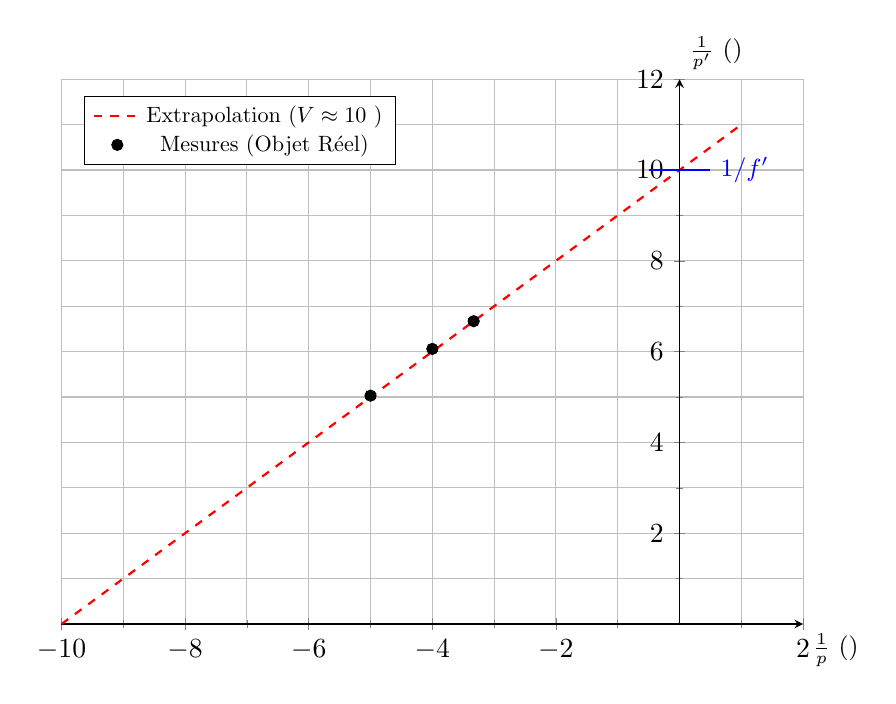
\begin{tikzpicture}
    \begin{axis}[
        axis lines = middle,
        xlabel = {$\frac{1}{p}$ (\unit{\per\meter})},
        ylabel = {$\frac{1}{p'}$ (\unit{\per\meter})},
        label style={font=\small},
        grid = both,
        minor tick num=1,
        xmin=-10, xmax=2,
        ymin=0, ymax=12,
        width=11cm, height=8.5cm,
        xlabel style={at={(ticklabel* cs:1)}, anchor=north west},
        ylabel style={at={(ticklabel* cs:1)}, anchor=south west},
        legend pos=north west,
        legend style={nodes={scale=0.8, transform shape}}
    ]

    % --- Extrapolation théorique ---
    \addplot[
        domain=-10:1,
        samples=2,
        thick,
        red,
        dashed,
    ] {x + 10};
    \addlegendentry{Extrapolation ($V \approx 10$ \unit{\per\meter})}

    % --- Points mesurés (Objet Réel) avec barres d'erreur ---
    \addplot[
        only marks,
        mark=*,
        black,
        error bars/.cd,
        y dir=both, y fixed=0.05,
        error mark options={rotate=90, mark size=2pt, line width=0.5pt}
    ]
    coordinates {
        (-5, 5.03)
        (-4, 6.06)
        (-3.33, 6.67)
    };
    \addlegendentry{Mesures (Objet Réel)}

    % --- Marquage de l'ordonnée à l'origine ---
    \draw[blue, thick] (axis cs:-0.5,10) -- (axis cs:0.5,10) node[right] {\small $1/f'$};

    \end{axis}
    \end{tikzpicture}
    \caption{Détermination de la vergence par exploitation de la relation de conjugaison.}
    \label{fig:graphe_focometrie}
\end{figure}

\subsubsection{Synthèse des résultats}
\begin{table}[H]
\centering
\caption{Résultat final de la distance focale de la lentille $L_1$}
\begin{tabular}{|p{3cm}|p{3cm}|}
\hline
\centering \textbf{$f_1'$ (cm)} & \centering \textbf{$\Delta f_1'$ (cm)} \tabularnewline \hline
\centering $10,0$ & \centering $0,1$ \tabularnewline \hline
\end{tabular}
\label{tab:E4_final}
\end{table}

\subsection{Méthode de Badal}

\subsubsection{Mesures brutes}
Au cours de l'expérience, nous avons relevé les mesures suivantes :
\begin{itemize}
    \item distance $d_1 = 20.0$ cm
    \item distance $d_2 = 60.0$ cm
\end{itemize}

\subsubsection{Calcul de la focale :}
En utilisant la relation démontrée précédemment :
\begin{equation}
    f'_{L'} = -\frac{(f'_{L2})^2}{d_2 - d_1} = -\frac{20,0^2}{60,0 - 20,0} = -10,0 \text{ cm}
\end{equation}

\subsubsection{Calcul d'incertitude :}
L'incertitude absolue $\Delta f'_{L'}$ est obtenue par la méthode de la différentielle totale. En considérant la focale de $L_2$ comme exacte, nous avons :
\begin{equation}
    \Delta f'_{L'} = |f'_{L'}| \cdot \frac{\Delta d_1 + \Delta d_2}{d_2 - d_1} = 10,0 \cdot \frac{0,2}{40,0} = 0,05 \text{ cm}
\end{equation}

\subsubsection{Tableau de synthèse :}
Le tableau suivant récapitule l'ensemble des grandeurs mesurées et calculées pour cette manipulation.

\begin{table}[h!]
    \centering
    \begin{tabular}{|c|c|c|c|c|}
        \hline
        $f'_{L2}$ (cm) & $d_1$ (cm) & $d_2$ (cm) & $f'_{L'}$ (cm) & $\Delta f'_{L'}$ (cm) \\
        \hline
        20,0 & 20,0 & 60,0 & -10,0 & 0,05 \\
        \hline
    \end{tabular}
    \caption{Détermination de la distance focale de la lentille divergente $L'$ par la méthode de Badal.}
\end{table}

